\documentclass[11pt,a4paper]{article}
\usepackage[margin=1in]{geometry}
\usepackage{amsmath}
\usepackage{booktabs}
\usepackage{graphicx}
\usepackage{fancyhdr}
\usepackage{hyperref}

\pagestyle{fancy}
\fancyhf{}
\lhead{Business Performance Analysis}
\rhead{Automated \LaTeX{} Report}
\cfoot{\thepage}

\title{Business Performance Analysis\\[2pt]\large Monthly Revenue, Expenses and Operating Profit}
\author{John Omole\\Mathematics and Statistics}
\date{October 28, 2026}

\begin{document}
\maketitle

\begin{abstract}
This report was generated automatically by a Python script from a CSV file.
It calculates operating profit and profit margin for each month, summarises
the year, draws a chart, and writes this \LaTeX{} document. The dataset is fictional.
\end{abstract}

\section{Methodology}
For each month $t$, operating profit, profit margin and revenue growth are
\begin{align}
P_t &= R_t - E_t, \\
M_t &= \frac{P_t}{R_t} \times 100\%, \\
G &= \frac{R_{\text{last}} - R_{\text{first}}}{R_{\text{first}}} \times 100\%.
\end{align}

\section{Data}
Table~\ref{tab:data} lists the monthly figures. All totals are computed by the
script from the rows shown, so they always agree with the table.

\begin{table}[h]
\centering
\caption{Monthly business performance}
\label{tab:data}
\begin{tabular}{lrrrr}
\toprule
Month & Revenue & Expenses & Profit & Margin \\
\midrule
January & 8,200 & 5,100 & 3,100 & 37.8\% \\
February & 9,100 & 5,400 & 3,700 & 40.7\% \\
March & 8,700 & 5,250 & 3,450 & 39.7\% \\
April & 10,300 & 5,900 & 4,400 & 42.7\% \\
May & 11,100 & 6,200 & 4,900 & 44.1\% \\
June & 11,800 & 6,500 & 5,300 & 44.9\% \\
July & 12,500 & 6,900 & 5,600 & 44.8\% \\
August & 12,100 & 6,750 & 5,350 & 44.2\% \\
September & 13,400 & 7,200 & 6,200 & 46.3\% \\
October & 14,100 & 7,600 & 6,500 & 46.1\% \\
November & 14,900 & 7,900 & 7,000 & 47.0\% \\
December & 15,800 & 8,300 & 7,500 & 47.5\% \\
\midrule
\textbf{Total} & \textbf{142,000} & \textbf{79,000} & \textbf{63,000} & \textbf{44.4\%} \\
\bottomrule
\end{tabular}
\end{table}

\section{Key Performance Indicators}
\begin{table}[h]
\centering
\caption{Annual performance indicators}
\begin{tabular}{lr}
\toprule
Indicator & Value \\
\midrule
Total revenue & 142,000 \\
Total expenses & 79,000 \\
Total operating profit & 63,000 \\
Average monthly revenue & 11,833 \\
Overall profit margin & 44.4\% \\
Revenue growth (January to December) & 92.7\% \\
\bottomrule
\end{tabular}
\end{table}

\section{Results}
Figure~\ref{fig:trend} shows the monthly movement of revenue, expenses and operating profit.

\begin{figure}[h]
\centering
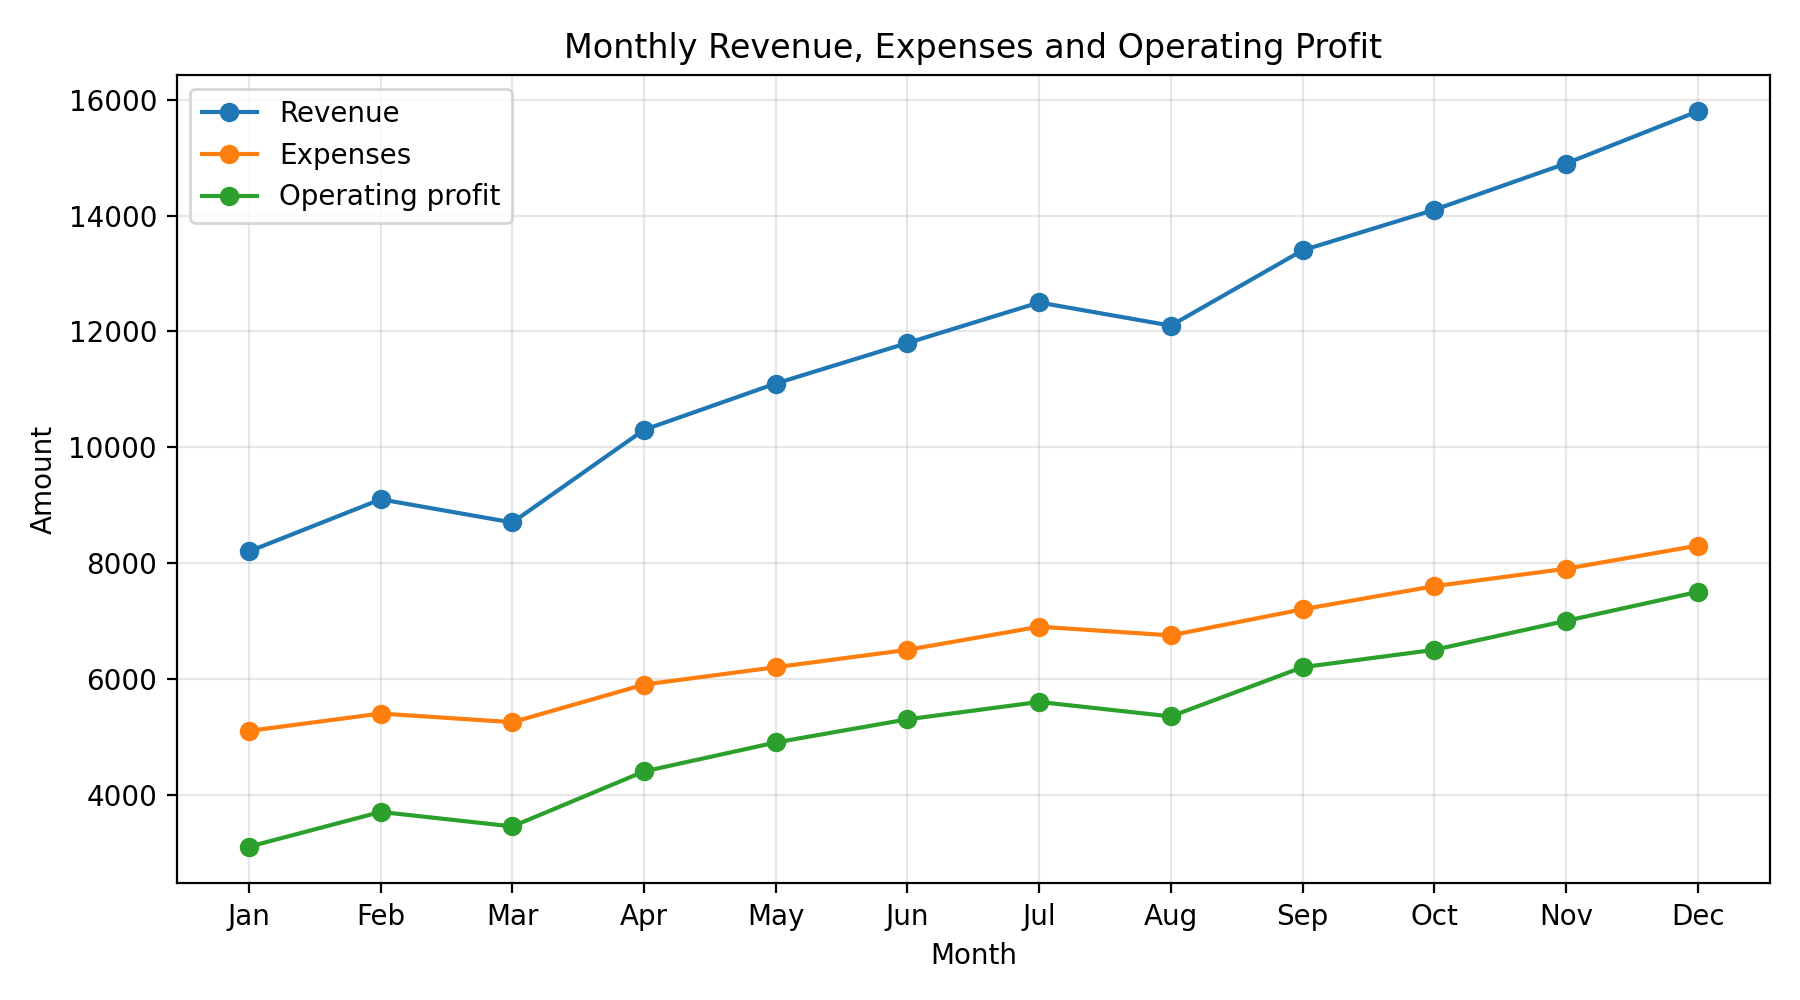
\includegraphics[width=0.9\textwidth]{chart.png}
\caption{Monthly revenue, expenses and operating profit}
\label{fig:trend}
\end{figure}

\section{Findings}
The following points were generated automatically from the data.
\begin{enumerate}
\item Revenue grew 92.7\% from January to December.
\item Total operating profit was 63,000, an overall margin of 44.4\%.
\item The most profitable month was December (7,500).
\item Revenue dipped compared with the previous month in: March, August.
\item Expenses stayed below revenue in every month.
\end{enumerate}

\section{Limitations}
The dataset is fictional and compact. It excludes taxes, depreciation,
financing costs, inflation adjustment and product-level detail.

\end{document}
